\documentclass[a4paper, 12pt]{article}
\usepackage{cite}
\usepackage{multicol, caption}
\usepackage{titling}
\usepackage{graphicx}
\usepackage{tabularx}
\usepackage{subcaption}
\usepackage{url}
\newenvironment{Figure}
  {\par\medskip\noindent\minipage{\linewidth}}
{\endminipage\par\medskip}

%加這個就可以設定字體
\usepackage{fontspec}
%使用xeCJK,其他的還有CJK或是xCJK
\usepackage{xeCJK}
\usepackage[margin=0.6in]{geometry}

%字型的設定可以使用系統內的字型,而不用像以前一樣另外安裝
\setCJKmainfont{DFKai-SB}
\author{}    
\newcommand*{\citenumfont}{}

% Reducing Distance of title and date
\setlength{\droptitle}{-2cm}
\title{\textbf{Offensive Tweet Classification}}
\renewcommand\maketitlehookc{\vspace{-3.5em}}


\begin{document}
    \maketitle     
    \begin{center}
        \begin{tabular}{ccc}
            陳君彥, b04703091 & 陳柔安, b04701232 & 蕭法宣, b04705007 \\
            b04703091@ntu.edu.tw &
            b04701232@ntu.edu.tw &
            b04705007@ntu.edu.tw
        \end{tabular}
    \end{center}

    \section*{Division of Work}
        陳君彥, b04703091: 
        \begin{itemize}
            \item Generation and testing of TFIDF-Vectorized models.
            \item Generation and testing of domain knowledge based features.
            \item Creation of written report.
        \end{itemize}
        陳柔安, b04701232:
        \begin{itemize}
            \item Generation and testing of bi-LSTM.
            \item Generation and testing of CNN models.
        \end{itemize}
        蕭法宣, b04705007:
        \begin{itemize}
            \item Generation and testing of BERT model.
            \item Generation and testing of string based features.
        \end{itemize}

    \section{Introduction}
        The goal of OffensEval competition on codalab by SemEval 2019 \cite{offens} is to tag a series of tweets with regards to their offensive nature. The competition is separated into 3 sub-tasks.
        \begin{itemize}
            \item Sub-task a: Tag a tweet based on whether the tweet is considered "offensive" or not. Tags include "OFF" and "NOT"
            \item Sub-task b: If a tweet is tagged as offensive in sub-task a, further tag the tweet on whether it is offensive in a targetted entity, or not targetted. Tags include "TIN" and "UNT".
            \item Sub-task c: If a tweet is tagged as targetted in sub-task b, further tag the tweet on whether it is targetted towards an individual, towards a group, or towards something else. Tags include "IND", "GRP", and "OTH".
        \end{itemize}

        \subsection{Dataset Analysis}
        
        \begin{center}
            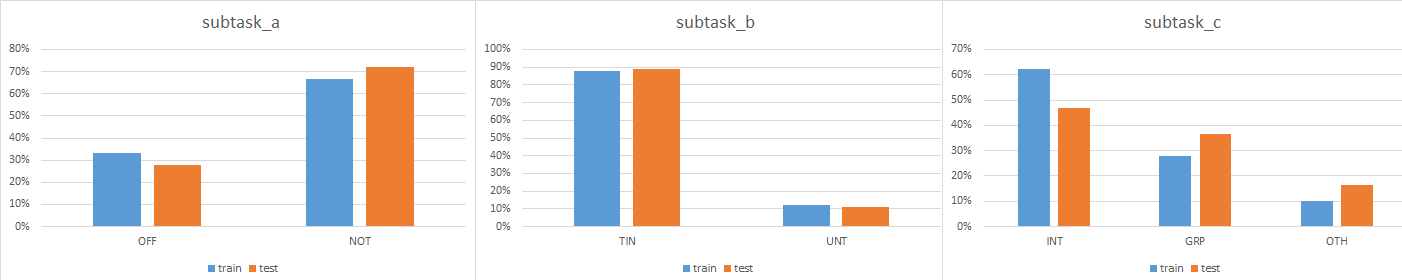
\includegraphics[width=\linewidth]{images/dist.png}
            \captionof{figure}{The percentage of each tag in the data set}
            \label{dist}
        \end{center}

        Our training dataset consists of 13240, 4400,  3876 tweets for sub-task a, b, c respectively, and the testing set has 620, 240, 213 respectively. We suspect the small size in the training data, coupled with the large disparity between the tag distribution as seen in Figure \ref{dist}, contributes greatly to the difficulty in creating an accurate prediction model.
        
    \begin{multicols}{2}

    \end{multicols}
    \newpage
    \section{Conclusion}
        We arrive at the conclusion that the aggregation of different features in our data is an effective method in indentifying and classifying fake news. After discussions with classmates and scouring forums for other people's attempt, we also conclude that this method is also rather efficient. 
        
        Our personal machines were all laptop spec'd machines, running the models within an acceptable time frame, with the results being only slightly lower than much more intensive models, such as BERT, which often require much more powerful hardware, and ran upwards of hours when training the models and predicting the results.

        \vskip 5cm
\bibliography{report}{}
\bibliographystyle{ieeetran}

\end{document}
